\documentclass[10pt,journal,compsoc]{IEEEtran}

%encoding
%--------------------------------------
\usepackage[T1]{fontenc}
\usepackage[utf8]{inputenc}
%--------------------------------------

\ifCLASSOPTIONcompsoc
  % IEEE Computer Society needs nocompress option
  % requires cite.sty v4.0 or later (November 2003)
  \usepackage[nocompress]{cite}
\else
  % normal IEEE
  \usepackage{cite}
\fi

\usepackage{graphicx}
\graphicspath{ {./images/} }

\usepackage{pgfplots}
\pgfplotsset{compat=1.15}

\hyphenation{op-tical net-works semi-conduc-tor}

\begin{document}

\title{An Approach for Game Engines Architecture}

\author{Felipe Gabriel de Oliveira Dias% <-this % stops a space
%\IEEEcompsocitemizethanks{\IEEEcompsocthanksitem M. Shell was with the Department
%of Electrical and Computer Engineering, Georgia Institute of Technology, Atlanta,
%GA, 30332.\protect\\
% note need leading \protect in front of \\ to get a newline within \thanks as
% \\ is fragile and will error, could use \hfil\break instead.
%E-mail: see http://www.michaelshell.org/contact.html
%\IEEEcompsocthanksitem J. Doe and J. Doe are with Anonymous University.}% <-this % stops an unwanted space
\thanks{Felipe Gabriel de Oliveira Dias, Computer Science Graduation Student at Universidade Tiradentes. Manuscript received December xx, 2019; revised xxxxxx xx, 2019.}}

% The paper headers
\markboth{xxxxxxxxxxxxx, December~2019}%
{}

\IEEEtitleabstractindextext{%
\begin{abstract}
If you want to create a game, a game engine is strictly necessary. There's a lot of game engines already in the market that can help the game development, but how about creating your own game engine, is that worth it? What difficulties will be in the development of a game engine? If you just want to create games, choose an already existing game engine is probably the right choice but create a game engine from scratch can be an interesting challenge to take. 
\end{abstract}

% Note that keywords are not normally used for peerreview papers.
\begin{IEEEkeywords}
Game Engine, Games, Software Architecture, Game Development
\end{IEEEkeywords}
}

\maketitle
\IEEEdisplaynontitleabstractindextext

\IEEEpeerreviewmaketitle

\IEEEraisesectionheading{\section{Introduction}\label{sec:introduction}}

\IEEEPARstart{V}{ideo} game development is not an easy task, before the 90', the game's source code was created exclusively for a single game, that way, source code reuse was really hard and create games by consequence. In the middle 90' Doom was launched by id Software. With a well-structured architecture, separating the main reusable components as rendering, audio player, physics simulation and others from the game-specific ones, the importance of a game engine was evident\cite{GameEngineArchitecture}. This article covers which features a game engine must have and how to architect it, and also covers the implementation of the Pluto Engine using the techniques described below and analyzes if creating a new game engine nowadays is worth it.

\hfill December xx, 2019
\section{What is a Game Engine?}
A game engine can be defined as an API\footnote{"In this case, “API” refers to “Application Programming Interface”, which at the level of a class, is defined by the set of exposed methods (whether “exposed” means public, documented of callable)."\cite{MendezBaudryMonperrus} "Modern software development is highly reliant on reusable APIs..."\cite{Bierhoff}.}, library\footnote{"Libraries provide pre-defined common functions to programmers for modular programming."\cite{Simsek}.} or framework\footnote{"Frameworks are of key importance for developing large-scale object-oriented software systems. They promise higher productivity and shorter time-to-market through design and code reuse." "Frameworks typically serve to implement (larger-scale) components, and are implemented using (smaller-scale) classes."\cite{FrameworkDesign}.} that makes the game development process easier, meaning that the most used game features were already implemented in a game engine such as memory management, resource management, rendering, physics simulation and others, that way the game developers can focus only on building the game mechanics itself\cite{3DGameEngineArchitecture}.

\subsection{Types of Game Engines}
Just like games, each game engine may focus on a different gender. The main reason for it is the efficiency of the features that the engine makes available to use. But some functionalities are developed in the same way every time, like rendering systems that can be shared between a lot of game genres. Other systems that can be reused are the audio player, physics simulator and so on.

\subsubsection{FPS}
First-person shooters had a great breakthrough in history, the first FPS games were located inside of corridors in order to have a good performance but nowadays they conquered large open worlds with incredible graphics. They are listed as the hardest game kind to produce, that's why some of the best technological advances in the game industry come from this kind. This kind of game focuses mostly on an efficient way to render large 3D virtual worlds, responsive camera control and some times small-scale online multiplayer capabilities\cite{GameEngineArchitecture}. Some of these games are: DOOM, Destiny, Titanfall, Half-Life and Overwatch\cite{FPSGames}.

\subsubsection{Racing}

\begin{figure}[!h] \centering \includegraphics[width=2.5in]{tree_a} \caption{"Opacity maps are popular for making layered billboard tree geometry. Use enough of
these and you’ll have a convincing forest if the camera is distant enough"\cite{AnIntroductionToComputerGraphicsForArtists}} \label{fig:racing-tree} \end{figure}

Racing games can be divided into two different sub-genres, the first one are the games that focus mainly on simulating a race and the other one are games that are not entirely focused on races but have vehicle mechanics as well. Apart from a different kind of gameplay, these games share a common thread, which is the physics-based simulation of racing\cite{AIGameEngineProgramming}. Some of the techniques used in racing game engines are rendering 2D elements for distant objects like tree as shown in figure \ref{fig:racing-tree}, hills and mountains, that why those games can improve their performance, one other technique divides the game world into 2D sectors, this can be used to improve performance when rendering elements and using artificial intelligence like pathfinders\cite{GameEngineArchitecture} as shown in figures \ref{fig:racing-path-a} and \ref{fig:racing-path-b}. Some famous racing game series are: Forza, Gran Turismo, Need for Speed, Mario Kart and Dirty\cite{RacingGames}.

\begin{figure}[!h] \centering \includegraphics[width=2.5in]{race_a} \caption{"Representation of a Racing Line"\cite{SearchingForTheOptimalRacingLineUsingGeneticAlgorithms}} \label{fig:racing-path-a} \end{figure}

\begin{figure}[!h] \centering \includegraphics[width=2.5in]{race_b} \caption{"An example of track decomposition process based on the intersection between the shortest path SP (reported as a blue line) and the minimum curvature path MCP (reported as a red line)."\cite{SearchingForTheOptimalRacingLineUsingGeneticAlgorithms}} \label{fig:racing-path-b} \end{figure}
\subsubsection{Fighting}
Fighting games generally focus on hand-to-hand combat, simulating real combats or even extrapolating the rules from the real world having crazy combos and effects. Some of the fighting games do not focus only on one vs one fights, that said, players can battle a lot of enemies at once, this kind of sub-genre is usually called beat 'em up\cite{FundamentalsOfGameDesign}. Game engines that focus on fighting games focus their technologies in fluid animations for the characters and physics collision precision\cite{GameEngineArchitecture}. Some famous fighting games are Street Fighter, Super Smash Bros, Mortal Kombat, Mother Russia Bleeds and Castle Crashers\cite{FightingGames,BeetEmUpGames}.

\subsubsection{Platform}
Platform games receives this name because in the platform games the player need to jump through platforms and reach the end of the stage. Due to hardware limitation, the early platform games were mostly 2D but with the technological advance, the genre also gain area between 3D games\cite{AIGameEngineProgramming}. Platform games mostly need a good scene editor that facilitates the creation of new stages, platforms and puzzles\cite{GameEngineArchitecture}. Some famous platform games are: Cuphead, Spyro, Shovel Knight, Sonic and Crash Bandicoot\cite{PlatformGames}.
\subsubsection{Strategy}
Strategy games creates a world that forces the players to think and achieve victory through planning. The main difference between puzzle games and strategy games is that in strategy games the player has opponents to battle against\cite{FundamentalsOfGameDesign}. "This definition distinguishes strategy games from puzzle games that call for planning in the absence of conflict, and from competitive construction and management
simulations that require planning but not direct action against an opponent."\cite{FundamentalsOfGameDesign}. Generally, strategy games use low-quality game elements to be able to have large quantities of elements in the scene and terrains usually use heightmap\footnote{"Height mapping (also known as parallax mapping) is a similar concept to normal mapping, however this technique is more complex - and therefore also more performance-expensive. Heightmaps are usually used in conjunction with normalmaps, and often they are used to give extra definition to surfaces where the texture maps are responsible for rendering large bumps and protrusions."\cite{UnityHeightMap}} based terrains\cite{GameEngineArchitecture}. Some famous strategy games are StarCraft, Red Alert, Stellaris, Civilization  and Total War\cite{StrategyGames}.

\begin{figure}[!h] \centering \includegraphics[width=2.5in]{heightmap_a} \caption{"This heightmap represents a 19.5km x 19.5km square."\cite{HeightmapRenderingUsingAFloorcastingAlgorithm}} \label{fig:heightmap-a} \end{figure}

\begin{figure}[!h] \centering \includegraphics[width=2.5in]{heightmap_b} \caption{A 3D representation of the heightmap presented in figure \ref{fig:heightmap-a} \cite{HeightmapRenderingUsingAFloorcastingAlgorithm}} \label{fig:heightmap-b} \end{figure}
\subsubsection{MMO}
Massively multiplayer online game or just MMO, can be any kind of game that support lots of players simultaneously in the same world. Generally MMOs are RPGs, but there's no rule that action games can't also be MMOs (e.g. Battle Royales). MMOs have the heavy lifting in the server side instead of the game engine, but a lots of optimizations can be made in the engine to avoid unnecessary requests to the server\cite{GameEngineArchitecture}. Some famous MMO games are: Ragnarok Online, Tibia, World of Warcraft, Player Unknown Battlegrounds and Fortnite\cite{MMOGames,BattleRoyaleGames}.
\subsection{Market}
These days there's a lot of game engines available in the market, each one has it's own business model, some of them requires a monthly payment for licensing, there are others that take some percentage of the game royalties, but there are also freemium\footnote{"A business model that allows a consumer to receive basic services for free, but requires them to pay for any service deemed to be premium. For instance, a cable provider may offer a customer free HBO for 2 weeks, but then require the customer to pay a fee for any program considered to be premium. Another example is computer software which offers a user basic use of the program, but requires a fee to access advanced features."\cite{Freemium}} and totally free game engines. In the next sections, this article will do a brief description from some famous game engines in the market.

\subsubsection{Unity}
According to itch.io\footnote{"itch.io is an open marketplace for independent digital creators with a focus on independent video games. It’s a platform that enables anyone to sell the content they've created."\cite{ItchIoAbout}.} today Unity is the most used game engine for free games development and independent companies in the market\cite{ItchIoEngines}. Had its release date back in 2005 by Unity Technologies, Unity enables game developers to create any kind of game for a variety of platforms like Microsoft Windows, Mac OS X, Nintendo Wii, iPhone/iPad, Xbox 360, Android, Windows Phone 8, PlayStation 3, PlayStation Vita, PlayStation 4, PlayStation Mobile, Adobe Flash Player, Linux, Nintendo Wii U, Gaikai, Xbox One, Nintendo Switch and others. Unity uses C\# as main scripting\footnote{"scripting was the kind of high-level programming that had always been envisioned, in the ascent from low-level assembly language programming to higher levels of abstraction:  it was concise, and it removed programmers from concerning themselves with many performance and memory management details;"\cite{Scripting}} language but in the past had support for Boo\footnote{"Boo is an object oriented, statically typed programming language for the Common Language Infrastructure, with a Python-inspired syntax and a special focus on language and compiler extensibility. Features such as type inference everywhere, duck typing on demand, pattern matching and syntactic macros are just a few of the special features Boo offers, in addition to the standard features a modern CLR developer expects (classes, structs, enums, generics, extension methods, async/await and so on.)"\cite{Boo}} and UnityScript\footnote{"UnityScript is a .NET-based dialect of JavaScript, so the syntax is similar to the popular web dialect of JavaScript. You will see it referred to as “UnityScript,” “JavaScript,” “Java Script,” and “Javascript” on the Unity web site and in the editor, but it is not same as JavaScript for web sites."\cite{UnityScript}}. Some games developed using Unity were: Days to Die, Angry Birds 2, Angry Birds Epic, Cities: Skylines, Cuphead, Deus Ex: The Fall, Escape from Tarkov, Fallout Shelter, Gris, Hearthstone: Heroes of Warcraft, Hollow Knight,  Kerbal Space Program, Oxygen Not Included, Pokémon GO, ReCore, Rust, Sonic Dash, Sonic Forces, Super Mario Run, Yandere Simulator, Monument Valley 2\cite{UnityGames}.
\subsubsection{Unreal}
Released in 1989 by Epic Games, Unreal Engine is a FPS focused game engine, but some games from different genders also has been developed using it. The main programming language is the C++, but the engine has support for a native system called Blueprints Visual Scripting that makes easier to develop games without the knowledge from programming languages but using diagrams instead. Just like Unity, the Unreal Engine can build games to a bunch of platforms such as Microsoft Windows, Linux, Mac OS, Mac OS X, Dreamcast, Nintendo GameCube, Nintendo Wii, Nintendo Wii U, Xbox, Xbox 360, Xbox One, PlayStation 2, PlayStation 3, PlayStation 4 and Nintendo Switch\cite{UnrealAbout}. Some games released using the engine were: Shadow Complex, Mass Effect, Unreal Tournament 3, Infinity Blade, Mirror’s Edge, Borderlands, Batman: Arkham Asylum, Gears of War, Enslaved: Odyssey to the West, Bioshock\cite{UnrealGames}.
\subsubsection{CryEngine}
 Just like the Unreal, CryEngine also focus in the FPS game genre, was initially developed for Nvidia\footnote{"NVIDIA awakened the world to the power of computer graphics when it invented the graphics processing unit (GPU) in 1999. 
Since then, it has consistently set new standards in visual computing with breathtaking, interactive graphics available on devices ranging from smart phones and tablets to notebooks and workstations."\cite{NvidiaAbout}} tech demos where was very successful. With the results, CryTek, the company who developed the engine began to make games with it. The first game series developed by the engine was FarCry in 2004. Only in 2011 the engine was open to the market with a licence that charges a fee from the game's revenue. The engine uses C++ and Lua as programming languages and can build games for some platforms such as: Microsoft Windows, Xbox 360, Xbox One, PlayStation 3, PlayStation 4 and Nintendo Wii\cite{CryEngineAbout}. Some games developed using the CryEngine were: Far Cry, Aion: The Tower of Eternity, Never Ending Dream, Crysis, WarFace, Ryse: Son of Rome, Sniper Ghost Warrior 2 and The Climb\cite{CryEngineGames}.
\subsubsection{Godot}
Godot is a free and open source\footnote{"The fundamental purpose of open source licensing is to deny anybody the right to exclusively exploit a work. Typically, in order to permit their works to reach a broad audience, and, incidentally, to make some sort of living from making works, creators are required to surrender all, or substantially all, of the rights granted by copyright to those entities that are capable of distributing and thereby exploiting that work."\cite{OpenSource}} game engine currently under the MIT licence\footnote{"The MIT License is short and to the point. It lets people do almost anything they want with your project, like making and distributing closed source versions."\cite{MIT}}. The engine focus both in 2D and 3D games and has support for several programming languages such as: C++, C\#, Rust, Nim, D and GDScript\footnote{"GDScript is a high level, dynamically typed programming language used to create content. It uses a syntax similar to Python (blocks are indent-based and many keywords are similar). Its goal is to be optimized for and tightly integrated with Godot Engine, allowing great flexibility for content creation and integration."\cite{GDScript}}. The engine can also compile for several platforms such: Microsoft Windows, Linux, Mac OS X, Android, iPhone/iPad and HTLM5\cite{GodotAbout} and some games developed using the engine were: Tanks of Freedom, Stereobreak, Steno Arcade, DeepSixed,Seek Etyliv, Grimante and Shipwreck\cite{GodotGames}.
\subsubsection{GameMaker}

\begin{figure*}[!t]
\centering
\subfloat{\includegraphics[width=6.5in]{dnd}} \caption{Game Maker Drag and Drop \cite{GameMakerDragNDrop}}
\label{fig:dnd}
\end{figure*}

GameMaker is a 2D game engine that was released with the objective to help the game development for developers that doesn't have prior experience in programming. GameMaker uses the DnD\footnote{"Drag and Drop (DnD™) is a visual scripting tool that can be used to create your games without actually typing any code."\cite{GameMakerDragNDrop}} as primary form of development as shown in figure \ref{fig:dnd}, but also has support for GML\footnote{"GameMaker: Studio has its own proprietary programming language called the GameMaker Language (abbreviated to GML)."\cite{GML}} as an alternative programming language\cite{TheGameMakerStandard}. Like the engines described in the sections above, the GameMaker can also make games for a bunch of platforms like Microsoft Windows, Mac OS X, Linux Ubuntu, Android, iPhone/iPad, tvOS, fireTV, Android TV, Microsoft UWP, HTML5, PlayStation 4 and Xbox One\cite{GameMaker}. Some games developed in the GameMaker were Hotline Miami, Gunpoint, Risk of Rain, Super Crate Box and Nuclear Throne\cite{TheGameMakerStandard}.

\subsubsection{Proprietary Engines}
There are many other game engines in the market, but some of then are in-house game engines, that is, only the company or partners has the licence to create games using these engines. Unreal and CryEngine started as in-house engines then later was made available for external use\cite{GameEngineArchitecture}. Some engines that retain in-house licence are the DICE Frostbite used by Electronic Arts to create the Battlefield series, Need for Speed series, Dragon Age and many others, Sage also by Electronic Arts is used to create real time strategy games, Rockstar Advanced Game Engine also known as RAGE is the engine used to create the Grand Theft Auto series, Red Dead Redemption series and Max Payne 3, Naughty Dog also has an in-house game engine used to create the The Last of Us series\cite{GameEngineArchitecture}.
\subsubsection{Pluto}\label{sec:pluto}
Pluto\cite{PlutoGitHub} is an open-source game engine developed by me and focuses on 2D games. In the section \ref{sec:game-egnine-architecture} is described how some of the systems that are already implemented in Pluto works. Pluto was developed using C++ as main language and is currently using a lot of third parties libraries to help the development process, the currently using libraries are OpenGL Mathematics\footnote{"OpenGL Mathematics (GLM) is a header only C++ mathematics library for graphics software based on the OpenGL Shading Language (GLSL) specifications."\cite{GLM}}, GLEW\footnote{"The OpenGL Extension Wrangler Library (GLEW) is a cross-platform open-source C/C++ extension loading library. GLEW provides efficient run-time mechanisms for determining which OpenGL extensions are supported on the target platform. OpenGL core and extension functionality is exposed in a single header file. GLEW has been tested on a variety of operating systems, including Windows, Linux, Mac OS X, FreeBSD, Irix, and Solaris."\cite{GLEW}}, GLFW\footnote{"GLFW is an Open Source, multi-platform library for OpenGL, OpenGL ES and Vulkan application development. It provides a simple, platform-independent API for creating windows, contexts and surfaces, reading input, handling events, etc."\cite{GLFW}}, \{fmt\}\footnote{"\{fmt\} is an open-source formatting library for C++. It can be used as a safe and fast alternative to (s)printf and iostreams."\cite{fmt}}, spdlog\footnote{"Very fast, header-only/compiled, C++ logging library."\cite{spdlog}}, Boost\footnote{"The Boost project provides free peer-reviewed portable C++ source libraries."\cite{boost}}, yaml-cpp\footnote{"yaml-cpp is a YAML parser and emitter in C++ matching the YAML 1.2 spec."\cite{yaml-cpp}}, stb\footnote{"single-file public domain (or MIT licensed) libraries for C/C++"\cite{stb}}, Box2D\footnote{"Box2D is an open source C++ engine for simulating rigid bodies in 2D. Box2D is developed by Erin Catto and has the zlib license."\cite{Box2DAbout}}, Conan\footnote{"The open source, decentralized and multi-platform package manager to create and share all your native binaries."\cite{conan}} and CMake\footnote{"CMake is an open-source, cross-platform family of tools designed to build, test and package software. CMake is used to control the software compilation process using simple platform and compiler independent configuration files, and generate native makefiles and workspaces that can be used in the compiler environment of your choice."\cite{CMake}}. Pluto has support for create 2D games with real-time physics simulation, in this article is shown a game that was developed using Pluto as game engine, a screenshot of the game can be seen in figure \ref{fig:pluto-flappy-bird}. Pluto is still a young project, not much more than half a year but is already in a stable state. Some of the features that Pluto already supports are file management, run-time asset loading (e.g. textures, meshes, materials, shaders, fonts and texts), 3D rendering, text rendering, real-time 2D physics, logging, external configuration loading, input management and 3D math library. In near future, the following features will be added to Pluto in the given order: compressed assets packages, python scripting support, audio player, visual editor and UI Manager. Pluto was only tested in Microsoft Windows but the project was designed to work both in Linux and Mac OS X as well.

\section{Game Engine Architecture}\label{sec:game-egnine-architecture}
In the sections bellow the main features from a game engine will be described in a architectural level and how software engineers can start a new game engine. The steps described will consider a bottom-up architecture but many times a game engine evolves through time in a way that we can't always predict new features for it, and it can make the source code become a spaghetti but with a good architecture this can be minimized\cite{TheCaseForResearchInGameEngineArchitecture, GameEngineArchitecture}.

\subsection{Core}
This section describes how game engines features can be abstracted for systems intercommunication and management.

\subsubsection{Memory Manager}
A game engine's memory manager is one of the most important features, not only algorithms but a bad memory management can cause high impact on the game performance\cite{GameEngineArchitecture}. Some common memory management implementations are using a Stack-based allocator, this way the engine can allocate a continuous memory segmentation, in C++ this can be achieved using the malloc native method\cite{GameEngineArchitecture, Malloc}. Others memory management techniques are the single frame memory or double-buffered frame memory and object pooling\cite{GameEngineArchitecture, MemoryAllocationPatternsUsedInGameDevelopment}.

\begin{figure}[!h] \centering \includegraphics[width=3in]{stack} \caption{A representation for stack allocation.\cite{GameEngineArchitecture}.} \label{fig:memory-stack} \end{figure}
\subsubsection{Services}
In this approach, services or subsystems are the most top abstraction level for the game engine features. Since a game engine has too many features a service pattern can help the start-up and shut-down process of the features. Each service can be represented as a singleton\footnote{"Ensure a class only has one instance, and provide a global point of access to it."\cite{GangOfFour}} and a service collection or a service locator\footnote{"Provide a global point of access to a service without coupling users to the concrete class that implements it."\cite{GameProgrammingPatterns}} can be implemented to help subsystems find each dependencies that is needed for them, sometimes a dependency injector\footnote{"Dependency Injection is a set of software design principles and patterns that enable us to develop loosely coupled code"\cite{DependencyInjectionIn.NET}} can be implemented for each service to help identify these dependencies. Services in this context are the memory manager, event manager, file system, resource manager and others\cite{GameEngineArchitecture,3DGameEngineArchitecture}.
\subsubsection{Events} \label{sec:events}
In order to prevent code coupling\footnote{"...the manner and degree of interdependence between software modules..."\cite{SystemsAndSoftwareEngineeringVocabulary}} a event queue\footnote{"A queue stores a series of notifications or requests in first-in, first-out order. Sending a notification enqueues the request and returns. The request processor then processes items from the queue at a later time. Requests can be handled directly or routed to interested parties. This decouples the sender from the receiver both statically and in time."\cite{GameProgrammingPatterns}} or event manager can be used to dispatch messages from one service to another, the service that dispatches the message doesn't know who gonna receive that message that is also valid for the receiver, the service doesn't know who sent the message. This pattern is also know as publish subscribe and can be used to make communication between services such an input manager sending an event when the user taps in some keyboard key to others services such as the game loop manager\cite{GameProgrammingPatterns, ZenjectSignals, GangOfFour} as shown in figure \ref{fig:pub-sub}.

\begin{figure}[!h] \centering \includegraphics[width=3in]{pub-sub} \caption{The representation diagram of a publish subscribe design pattern\cite{pub-sub}.} \label{fig:pub-sub} \end{figure}

\subsection{File System}
Manipulating files is a primordial feature for a game engine, the file system is responsible for all I/O file operations. The main functionalities that the file system must provide is to translate paths between operating systems such as Windows and Unix, manage files and folders contents, be able to read and write files in a asynchronous way for better performance. File systems generally provide a set of methods for open, close, read, write files\cite{GameEngineArchitecture}.
\subsection{HID Manager}
Almost all games must have a interaction with the player, to that work a game engine must manage the human interfaces devices (HID) connected to be able to receive inputs from players\cite{GameEngineArchitecture}. There are several kinds of input devices such as Joysticks, Keyboard and Mouses, the engine must receive and handle those inputs and redirect those commands for the correct place, the redirection can be implemented using the event system described in the section \ref{sec:events}\cite{GameProgrammingPatterns}. Several input events can come from a single game frame, so the HID manager must keep a pool of those inputs that has fired in that specific frame and dispatch them in the right moment\cite{GameEngineArchitecture}. There are some types of input data such as buttons that are generally treated as on and off and analog stickers that can be treated as 2D vectors containing the positions for both vertical and horizontal axis. The main functionalities that a HID manager must provide are input dead zones\footnote{"Dead zones are simply a minimum input threshold, often somewhere between 0.1 to 0.2. If the input received from the stick is smaller than that, it’s ignored."\cite{DeadZones}}, analog signal filtering, input event detection, management of multiple HIDs for multiple players, multi-platform HID support and controller input remapping that can be done using the command\footnote{"Encapsulate a request as an object, thereby letting users parameterize clients with different requests, queue or log requests, and support undoable operations."\cite{GameProgrammingPatterns}} design pattern\cite{GameEngineArchitecture, GameProgrammingPatterns}.
\subsection{Resources}
Games need a bunch of elements that are specific for each kind of game, these elements can be called resources or even assets. Some of theses assets are 3D models, material\footnote{"In the real world, each object reacts differently to light. Steel objects are often shinier than a clay vase for example and a wooden container does not react the same to light as a steel container. Each object also responds differently to specular highlights. Some objects reflect the light without too much scattering resulting in a small highlights and others scatter a lot giving the highlight a larger radius."\cite{LearnOpenGL}}, images, shaders\footnote{"The current state of the art in real-time computer graphics is programmable shading."\cite{OpenGLBible}}, animations and much more\cite{UnityResources}. It's a game engine responsibility to manage all those resources in run-time. Some game engines creates it's own asset file format, this way the engine can load the assets faster, since it's an already known format. In order to this work, the game engine needs to compute these assets from native formats (e.g. .PNG for images, .OBJ for 3D models) to a internal one during the game development. The resource manager must ensures that assets only have one unique instance in memory, must control resources lifetime and identify when each asset can be safely disposed. One big responsibility is to keep referential integrity, so if assets reference one another, they can be unloaded then reloaded and the game must be like the initial state\cite{GameEngineArchitecture}.
\subsection{Game Loop}
Just like real life, time has great importance for games as well. In a game there's too many things happening at once, so it's the game loop manager responsibility to keep all of those subsystems synchronized\cite{GameEngineArchitecture, GameProgrammingPatterns}. Scenes behaviours can be updated every game loop differently from rendering that must keep synchronized with the user's monitor (e.g. 30hz or 60hz). Physics simulation needs a more frequent update (e.g. 120hz) from the rendering to keep the simulation more fluid\cite{GameEngineArchitecture}. In a naive approach, game loop manager also known as simulation manager can be easily implemented using the programming while operation, while the game is running, all subsystems will be updated according to its priority, generally, the priority order is input manager, scene manager, physics manager and render manager\cite{GameProgrammingPatterns} an example can be seen in figure \ref{fig:game-loop}.

\begin{figure}[!h] \centering \includegraphics[width=3in]{game-loop} \caption{A game loop example diagram.\cite{GameProgrammingPatterns}.} \label{fig:game-loop} \end{figure}
\subsection{Scene}
When you are making a game, even a small one, there's a lot of objects running at the same time, these objects can be 3D models, Sprites, UI Elements and more\cite{ObjectOrientedGameProgrammingTheSceneSystem}. In order to render be effective, the scene manager needs to keep track of the in-game object that is currently composing the scene. A naive approach to the problem is iterate over all objects in the scene and then render it, but this approach doesn't have a good performance at all, since even objects that are not in the camera view will be rendered as well, one good solution for the problem is to implement a scene graph\footnote{"Abstractly put, a Scene Graph is an organized hierarchy of nodes in a data structure with special relationships that simplify a problem.", "A Scene Graph is an m-ary tree, a tree with any node possessing any number of children, in which any particular node will inherit and amalgamate the transformations and render states, or other such states of the parent."\cite{ObjectOrientedSceneManagement}}, this way only objects and it's children that are visible to the camera can be rendered\cite{3DGameEngineDesign}.

\begin{figure*}[!t]
\centering
\subfloat{\includegraphics[width=6.5in]{scene-graph}} \caption{Scene graph representation in a photograph \cite{SceneGraphRepresentationAndLearning}.}
\label{scene-graph}
\end{figure*}
\subsection{Rendering}
This probably is the most important feature for modern game engines, rendering is a really big topic to cover\cite{GameEngineArchitecture} and has become one of the most difficult software engineer project to be working with due to a large number of complex algorithms\cite{DesigningAModernRenderingEngine}. The render manager has the responsibility to send the information from the game scene to the player monitor, so it's responsible for the communication with the GPU, luckily, there's some APIs available that do a perfect job for this (e.g. OpenGL\footnote{"OpenGL is strictly defined as “a software interface to graphics hardware.” In essence, it is a 3D graphics and modeling library that is highly portable and very fast. Using OpenGL, you can create elegant and beautiful 3D graphics with exceptional visual quality. The greatest advantage to using OpenGL is that it is orders of magnitude faster than a raytracer or software rendering engine."\cite{OpenGLBible}}, DirectX\footnote{"Direct3D 12 is a rendering library for writing high-performance 3D graphics applications using modern graphics hardware on various Windows 10 platforms (Windows Desktop, Mobile, and Xbox One). Direct3D is a low-level library in the sense that its application programming interface (API) closely models the underlying graphics hardware it controls. The predominant consumer of Direct3D is the games industry, where higher level rendering engines are built on top of Direct3D."\cite{DirectX}} and Metal\footnote{"In 2014, Apple introduced a new low-level GPU programming framework for iOS: Metal. A year later, Metal came to macOS, followed by watchOS and tvOS. Apple devices have two “brains” that can be programmed to create applications: a central processing unit (CPU) and a graphics processing unit (GPU). The GPU is a specialized processor that does floating-point math in parallel very quickly and efficiently. These tasks are expensive on the CPU because they can’t be done in parallel, so various frameworks and APIs have been created to offload these expensive tasks to the processor that is best equipped to do them."\cite{Metal}}). It changes the way how the render manager will work if the game engine focus in a multi-platform development, because it now needs to choose the correct API for each operating system such as DirectX if the game is running on Windows, OpenGL if Linux or Android and Metal for Mac and iOS devices. It's also the responsibility of the render manager to manage the assets in the GPU's memory, so resources like textures, shaders and meshes\footnote{"In order to generate the necessary geometry for realtime rendering of subdivision surfaces, complete topology information is necessary for a given mesh of input polygons. Over the years a number of mesh representations have been developed that provide this topology information, given an arbitrary input mesh."\cite{AMeshDataStructureForRenderingAndSubdivision}} are not misused. Bake multiple meshes as a single one to reduce draw calls\footnote{"To draw a GameObject on the screen, the engine has to issue a draw call to the graphics API (such as OpenGL or Direct3D). Draw calls are often resource-intensive, with the graphics API doing significant work for every draw call, causing performance overhead on the CPU side. This is mostly caused by the state changes done between the draw calls (such as switching to a different Material), which causes resource-intensive validation and translation steps in the graphics driver."\cite{UnityDrawCall}} to the GPU since it has a high cost for performance.
\subsection{Physics}
Just like the Rendering system, the Physics simulation has a world for itself and most AAA\footnote{AAA is oftenly used in game industry to represent high budget games.} games have a physics simulation in it, so for achieving a good quality game, a physics simulation must be integrated within the engine\cite{GamePhysicsEngineDevelopment}. Some features that a game engine with physics simulation should provide are a collision detection between static and dynamic scene objects, simulate rigid bodies over the influence of external forces and gravity, string-mass simulation, ray and shape casts, volume triggers, vehicle simulation with realistic suspensions, rag dolls and much more\cite{GameEngineArchitecture}. Since a physics system could be considered a whole project for itself, when creating a game engine you should consider using already existing physics engines like Box2D, PhysX\footnote{"The NVIDIA PhysX SDK is a scalable multi-platform physics solution supporting a wide range of devices, from smartphones to high-end multicore CPUs and GPUs. PhysX is already integrated into some of the most popular game engines, including Unreal Engine, and Unity3D."\cite{PhysXAbout}} or Havok\footnote{"Havok Physics offers the fastest, most robust collision detection and physical simulation technology available, which is why it has become the gold standard within the games industry and has been used by more than half of the top selling titles this console generation."\cite{HavokAbout}}\cite{PhysicsForGameDevelopers}. So the game engine needs to integrate one or many of those physics engines with other services such as the scene manager to know where which object is and updates its position and the render manager to be able to debug physics data.

\begin{figure}[!h] \centering \includegraphics[width=2.5in]{physics-contact} \caption{2D Physics contact points and circle move direction\cite{GameEngineArchitecture}.} \label{fig:physics-contact} \end{figure}
%\subsection{Debug}

\input{sections/architecture/debug/logs.tex}
\input{sections/architecture/debug/gizmos.tex}

\section{Benchmark}

\begin{figure*}[!h]
\centering
\subfloat[Pluto]{\includegraphics[width=1.6in]{pluto-flappy-bird} \label{fig:pluto-flappy-bird}}
\hfil \subfloat[Unity]{\includegraphics[width=1.6in]{unity-flappy-bird} \label{fig:unity-flappy-bird}} \caption{Flappy Bird developed using Pluto and Unity} \label{fig:flappy-bird}
\end{figure*}

In this section, a benchmark between two engines will be shown, one engine will be using the techniques described in the sections below, the engine described in section \ref{sec:pluto} and the other one is the Unity, I'm choosing the Unity because I already have almost a decade of experience in it. For the benchmark, two games were developed using the engines, the game is a copy of Flappy Bird\footnote{"...Flappy Bird, developed by Gears Studio the concept is a simple, you have to tap a bird to make it fly and try to maneuver it through different obstacles the further you reach the higher your score will be being each obstacle 1 point."\cite{FlappyBird}} as shown in figure  \ref{fig:flappy-bird}. No specific optimizations were done for the chosen game but for the Unity the game will be compiled using both Mono\footnote{"Mono is an open source implementation of Microsoft's .NET Framework based on the ECMA standards for C\# and the Common Language Runtime."\cite{Mono}} and IL2CPP\footnote{"IL2CPP (Intermediate Language To C++) is a Unity-developed scripting backend which you can use as an alternative to Mono when building projects for various platforms. When building a project using IL2CPP, Unity converts IL code from scripts and assemblies to C++, before creating a native binary file (.exe, apk, .xap, for example) for your chosen platform. Some of the uses for IL2CPP include increasing the performance, security, and platform compatibility of your Unity projects."\cite{IL2CPP}} as scripting backend. All tests were run in the same environment, an Alienware 15 R3, Windows 10 64-bit, Intel i5-7300HQ CPU @ 2.5GHz, 32GB 2400MHz RAM, GTX 1060 6GB GPU and 500GB Samsung SSD 960 Evo. As shown in Mishra and Shrawankar's paper, this article will take benchmarks on CPU utilization, GPU utilization, frames per second and memory utilization\cite{ComparisonBetweenFamousGameEnginesAndEminentGames} as well the application load time and size in the disk.

\subsection{Development}
The development process is also an important thing to measure, since the implementation of the engine took more than half a year to reach this stable state and an additional week to develop the game, it was entirely developed in the source code without any visual editor tool to help the development. On the other hand, Unity is already available in the market and has an awesome visual editor to build games. With the Unity built-in tools were possible to develop the same game in almost four hours. So since unity already holds a bunch of features to help the game development, they won this one.
\subsection{Performance}
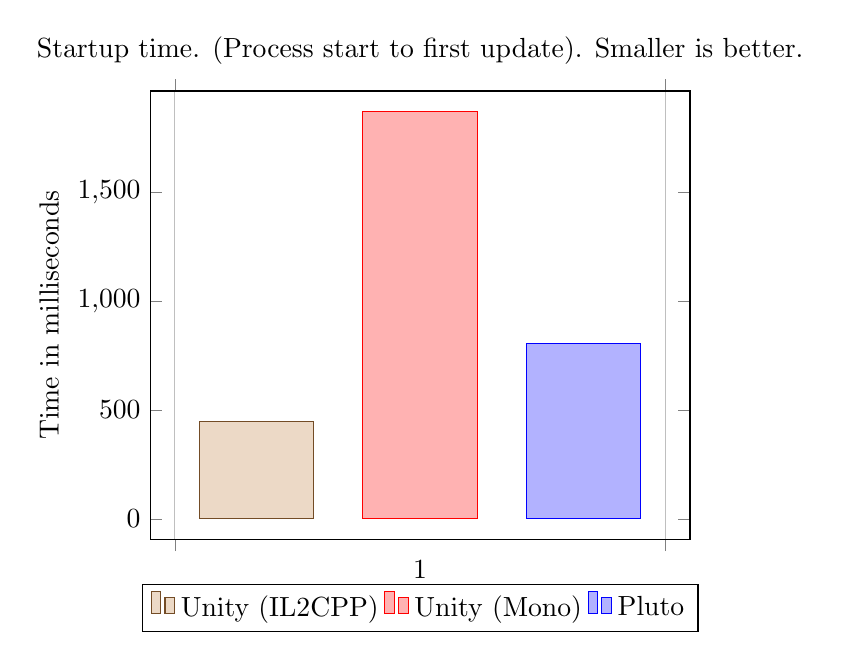
\begin{tikzpicture}
\begin{axis}[
    title={Startup time. (Process start to first update). Smaller is better.},
    reverse legend,
	x tick label style={
		/pgf/number format/1000 sep=},
	ylabel=Time in milliseconds,
	enlargelimits=0.05,
	legend style={at={(0.5,-0.1)},
	anchor=north,legend columns=-1},
	ybar interval=0.7,
]
\addplot 
	coordinates {(1,805) (0,0)};
\addplot 
	coordinates {(1,1870) (0,0)};
\addplot 
	coordinates {(1,445) (0,0)};
\legend{Pluto,Unity (Mono), Unity (IL2CPP)}
\end{axis}
\end{tikzpicture}
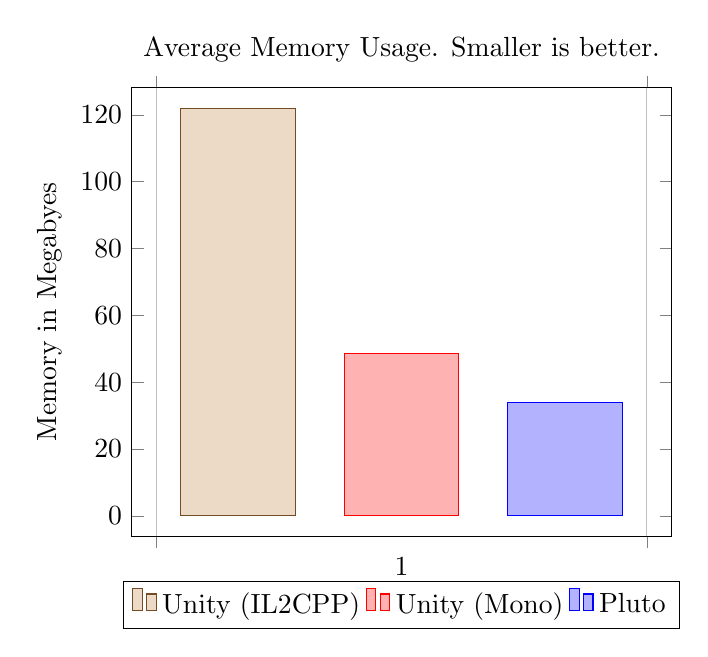
\begin{tikzpicture}
\begin{axis}[
    title={Average Memory Usage. Smaller is better.},
    reverse legend,
	x tick label style={
		/pgf/number format/1000 sep=},
	ylabel=Memory in Megabyes,
	enlargelimits=0.05,
	legend style={at={(0.5,-0.1)},
	anchor=north,legend columns=-1},
	ybar interval=0.7,
]
\addplot 
	coordinates {(1,34) (0,0)};
\addplot 
	coordinates {(1,48.5) (0,0)};
\addplot 
	coordinates {(1,122) (0,0)};
\legend{Pluto,Unity (Mono), Unity (IL2CPP)}
\end{axis}
\end{tikzpicture}
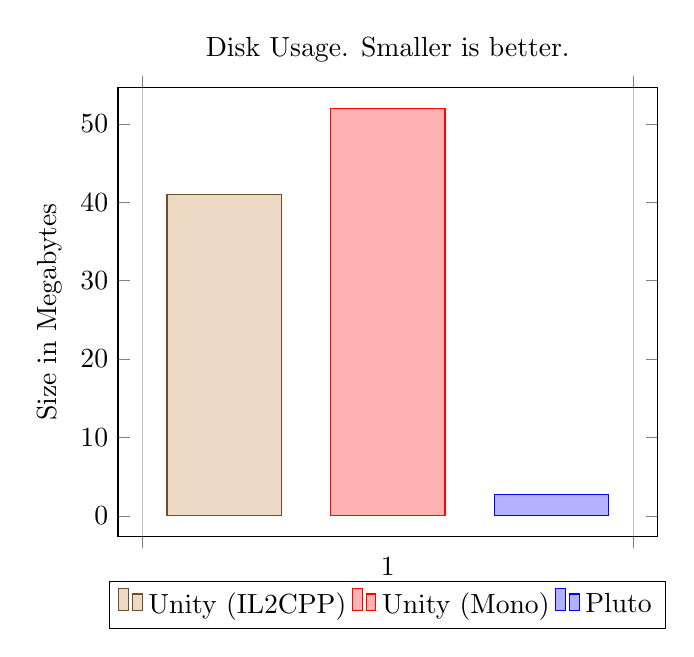
\begin{tikzpicture}
\begin{axis}[
    title={Disk Usage. Smaller is better.},
    reverse legend,
	x tick label style={
		/pgf/number format/1000 sep=},
	ylabel=Size in Megabytes,
	enlargelimits=0.05,
	legend style={at={(0.5,-0.1)},
	anchor=north,legend columns=-1},
	ybar interval=0.7,
]
\addplot 
	coordinates {(1,2.67) (0,0)};
\addplot 
	coordinates {(1,52) (0,0)};
\addplot 
	coordinates {(1,41) (0,0)};
\legend{Pluto,Unity (Mono), Unity (IL2CPP)}
\end{axis}
\end{tikzpicture}
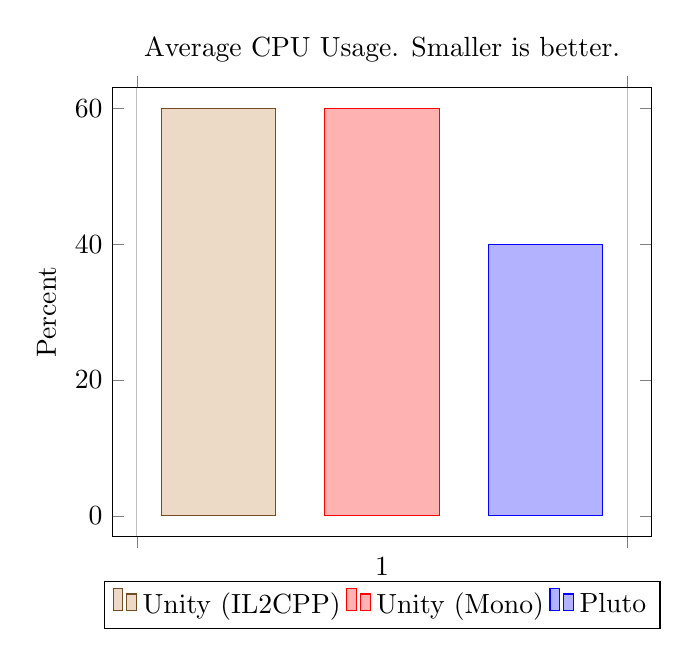
\begin{tikzpicture}
\begin{axis}[
    title={Average CPU Usage. Smaller is better.},
    reverse legend,
	x tick label style={
		/pgf/number format/1000 sep=},
	ylabel=Percent,
	enlargelimits=0.05,
	legend style={at={(0.5,-0.1)},
	anchor=north,legend columns=-1},
	ybar interval=0.7,
]
\addplot 
	coordinates {(1,40) (0,0)};
\addplot 
	coordinates {(1,60) (0,0)};
\addplot
	coordinates {(1,60) (0,0)};
\legend{Pluto,Unity (Mono), Unity (IL2CPP)}
\end{axis}
\end{tikzpicture}
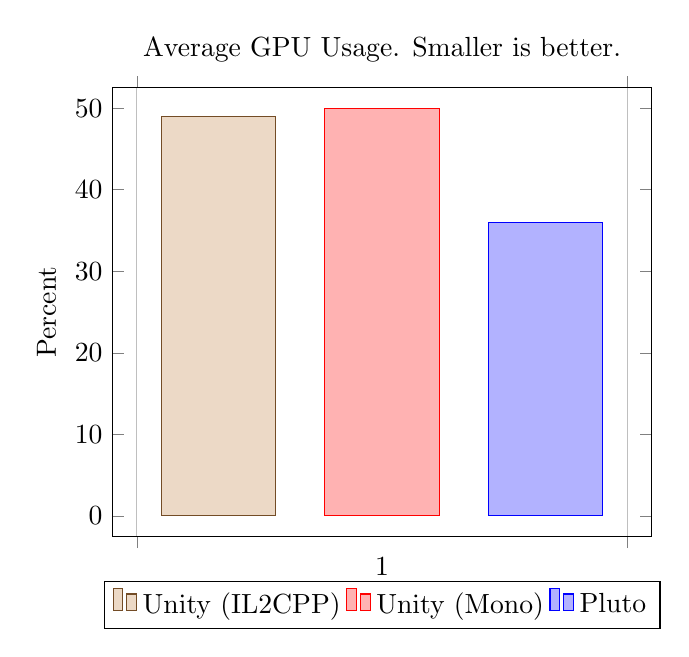
\begin{tikzpicture}
\begin{axis}[
    title={Average GPU Usage. Smaller is better.},
    reverse legend,
	x tick label style={
		/pgf/number format/1000 sep=},
	ylabel=Percent,
	enlargelimits=0.05,
	legend style={at={(0.5,-0.1)},
	anchor=north,legend columns=-1},
	ybar interval=0.7,
]
\addplot 
	coordinates {(1,36) (0,0)};
\addplot 
	coordinates {(1,50) (0,0)};
\addplot 
	coordinates {(1,49) (0,0)};
\legend{Pluto,Unity (Mono), Unity (IL2CPP)}
\end{axis}
\end{tikzpicture}
\begin{tikzpicture}[step y=500]
\begin{axis}[
    title={Average Frames per Second. Higher is better.},
    reverse legend,
	x tick label style={
		/pgf/number format/1000 sep=},
	ylabel=FPS,
	enlargelimits=0.05,
	legend style={at={(0.5,-0.1)},
	anchor=north,legend columns=-1},
	ybar interval=0.7,
]
\addplot 
	coordinates {(1,2632) (0,0)};
\addplot 
	coordinates {(1,2455) (0,0)};
\addplot
	coordinates {(1,3024) (0,0)};
\legend{Pluto,Unity (Mono), Unity (IL2CPP)}
\end{axis}
\end{tikzpicture}

\section{Conclusion}
Despite the efforts to create a new game engine from scratch its still have several performance issues, and even Unity supporting a lot of awesome features it still beats Pluto from both FPS and load times, but we can notice that Pluto is not using the same Memory, CPU and GPU usage as Unity, so there's a lot of room for improvements in there but that would take more time to implement it. As well for the size of the application, we can see that Unity has a lot of footprint for a basic game such as Flappy Bird and if you think in community support Pluto totally lack of it and Unity has one of the largest communities in the game engine industry, in the other hand, game developers need to keep up with Unity feature schedule that can delay the implementation of new features and bug corrections. So if you just want to create games, the benchmarks shown in this article suggests that using an engine already established in the market will increase the chances for better result because that will be much less time consuming and the development team can focus only in the game logic itself then creating a new engine from scratch, unless the goal is to study how game engines work or it is a big company that wants to take control of every little bit in their games.

\section*{Acknowledgments}
I would like to thank Felipe Goulart for been a great mentor when I started working at Lumen Games (Lumentech back in 2012) and now as professor helping me to finish my B.S. degree. Also I would like to thank my Mom, Dad and Sister for support me in this long road that I take for last I thank to all my colleagues in Lumen Games the ones that's are currently working there and the ones that already left for helping me develop my abilities to be a better person and as well a software engineer.

\ifCLASSOPTIONcaptionsoff
  \newpage
\fi

% references section

\begin{thebibliography}{1}

\bibitem{GameEngineArchitecture}
J. Gregory, Game Engine Architecture. 3rd ed. USA: CRC Press, 2019.

\bibitem{MendezBaudryMonperrus}
D. Mendez, B. Baudry, M. Monperrus, Empirical Evidence of Large-Scale Diversity in API Usage of Object-Oriented Software, in International Conference on Source Code Analysis and Manipulation, Eindhoven, 2013, pp. 10, 10.1109/SCAM.2013.6648183.

\bibitem{Bierhoff}
K. Bierhoff, "API Protocol Compliance in Object-Oriented Software," Ph.D. dissertation, Institute for Software Research, School of Computer Science, Carnegie Mellon University, Pittsburgh, 2009.

\bibitem{Simsek}
B. Simsek, "How To Create Program Libraries," Aug 18 2004.

\bibitem{FrameworkDesign}
D. Riehle, "Framework Design: A Role Modeling Approach," ETH Zürich, Dissertation Nr. 13509, 2000.
 
\bibitem{3DGameEngineArchitecture} 
D. Eberly, 3D Game Engine Architecture: Engineering Real-Time Applications with Wild Magic, USA: Elsevier Inc, 2005.

\bibitem{AnIntroductionToComputerGraphicsForArtists}
A. Paquette, An Introduction to Computer Graphics for Artists, 2nd ed. London: Springer, 2013.

\bibitem{FPSGames}
GamesRadar+ (2018) The 25 best FPS game of all time. [Online]. Available: https://www.gamesradar.com/best-fps-games/3/

\bibitem{AIGameEngineProgramming}
B. Schwab, AI Game Engine Programming, 2nd ed. Boston, 2009. 

\bibitem{RacingGames}
Ranker (2019) The 20+ Most Popular Racing Games in 2019. [Online]. Available: https://www.ranker.com/list/most-popular-racing-video-games-today/ranker-games

\bibitem{SearchingForTheOptimalRacingLineUsingGeneticAlgorithms}
L. Cardamone, D. Loiacono, P. L. Lanzi and A. P. Bardelli. "Searching for the Optimal Racing Line Using Genetic Algorithms," in Computational Intelligence and Games, 2010, doi. 388 - 394. 10.1109/ITW.2010.5593330. 

\bibitem{FundamentalsOfGameDesign}
E. Adams, Fundamentals of Game Design, 2nd ed. Berkeley, 2010

\bibitem{FightingGames}
Game Informer (2019) The 30 Greatest Fighting Games of All Time. [Online]. Available: https://www.gameinformer.com/2019/04/25/the-30-greatest-fighting-games-of-all-time

\bibitem{BeetEmUpGames}
PC Gamer (2018) The best beat-em-ups on PC. [Online]. Available: https://www.pcgamer.com/best-beat-em-up-games/

\bibitem{PlatformGames}
PCGamesN (2019) The best platform games on PC. [Online]. Available: https://www.pcgamesn.com/best-platform-games

\bibitem{UnityHeightMap}
Unity (2020) Manual: Heightmap. [Online]. Available: https://docs.unity3d.com/Manual/StandardShaderMaterialPara
meterHeightMap.html

\bibitem{StrategyGames}
PC Gamer (2019) Best Strategy Games on PC. [Online]. Available: https://www.pcgamer.com/the-best-strategy-games/

\bibitem{HeightmapRenderingUsingAFloorcastingAlgorithm}
Observable (2018) Heightmap rendering using a floorcasting algorithm. [Online]. Available: https://observablehq.com/@ehouais/heightmap-rendering-using-a-floorcasting-algorithm

\bibitem{MMOGames}
MMORPG (2019) MMORPG Game List 2019. [Online]. Available: https://www.mmorpg.com/games-list

\bibitem{BattleRoyaleGames}
PC Gamer (2019) The Battle Royale Games of 2019. [Online]. Available: https://www.pcgamer.com/battle-royale-games-2018/

\bibitem{Freemium}
Business Dictionary (2019) What is freemium? Definition and meaning. [Online]. Available: http://www.businessdictionary.com/definition/freemium.html

\bibitem{ItchIoAbout}
Itch.io (2019) About itch.io. [Online]. Available: https://itch.io/docs/general/about

\bibitem{ItchIoEngines}
Itch.io (2019) Most used Engines. [Online]. Available: https://itch.io/game-development/engines/most-projects

\bibitem{Scripting}
R. P. Loui, "In Praise of Scripting: Real Programming Pragmatism," [Online], Jan, 10, 2012, Available: https://steloflute.tistory.com/389

\bibitem{Boo}
Mono (2017) Boo [Online]. Available: https://www.mono-project.com/archived/boo/

\bibitem{UnityScript}
J. Suvak, Learn Unity3D Programming with UnityScript: Unity’s JavaScript for Beginners, USA: Apress, 2014.

\bibitem{UnityGames}
Unity (2019) Made With Unity. [Online]. Available: https://unity.com/madewith

\bibitem{UnrealAbout}
Unreal Engine (2019) Features. [Online]. Available: https://www.unrealengine.com/en-US/features

\bibitem{UnrealGames}
Techtudo (2011) Top 10: \textit{O mais belos games com} Unreal Engine 3 [Online]. Available: https://www.techtudo.com.br/noticias/noticia/2011/02/top-10-o-mais-belos-games-com-unreal-engine-3.html

\bibitem{NvidiaAbout}
NVidia (2019) Company Overview. [Online]. Available: https://www.nvidia.com/en-us/drivers/citizenship-report-company-overview/

\bibitem{CryEngineAbout}
CRYENGINE (2019) Features. [Online]. Available: https://www.cryengine.com/features

\bibitem{CryEngineGames}
CryEngine (2019) All the games created by video game developer Crytek. [Online]. Available: https://www.crytek.com/games>

\bibitem{OpenSource}
A. M. Laurent, Understanding Open Source and Free Software Licensing, USA: O'Reilly Media, 2004.

\bibitem{MIT}
Choose a License (2019) Choose an open source license. [Online]. Available: https://choosealicense.com/

\bibitem{GDScript}
Godot Engine. (2018) GDScript the Godot Engine lastest documentation. [Online]. Available: http://docs.godotengine.org/en/3.0/getting\_started/scripting
/gdscript/gdscript\_basics.html

\bibitem{GodotAbout}
OpenHub (2019) The Godot Game Engine Open Source Project on Open Hub. [Online]. Available: https://www.openhub.net/p/godotengine

\bibitem{GodotGames}
Godot Engine (2019) Showcase. [Online]. Available: https://godotengine.org/showcase

\bibitem{GameMakerDragNDrop}
YoYoGames (2019) Drag And Drop Overview. [Online]. Available: https://docs2.yoyogames.com/source/\_build/3\_scripting/1\_drag
\_and\_drop\_overview/index.html

\bibitem{GML}
YoYoGames (2019) GLM Overview. [Online]. Available: https://docs.yoyogames.com/source/dadiospice/002\_reference
/001\_gml\%20language\%20overview/

\bibitem{TheGameMakerStandard}
D. V. Vinciguerra and A. Howell, The GameMaker Standard. USA: CRC Press, 2016.

\bibitem{GameMaker}
YoYoGames (2019) GameMaker. [Online]. Available: https://www.yoyogames.com/gamemaker

\bibitem{PlutoGitHub}
GitHub (2019) pluto. [Online]. Available: https://github.com/felipegodias/pluto

\bibitem{GLM}
GitHub (2019) OpenGL Mathematics. [Online]. Available: https://github.com/g-truc/glm

\bibitem{GLEW}
GitHub (2019) The OpenGL Extension Wrangler Library. [Online]. Available: https://github.com/nigels-com/glew

\bibitem{GLFW}
GitHub (2019) A multi-platform library for OpenGL, OpenGL ES, Vulkan, window and input. [Online]. Available: https://github.com/glfw/glfw

\bibitem{fmt}
GitHub (2019) A modern formatting library. [Online]. Available: https://github.com/fmtlib/fmt

\bibitem{spdlog}
GitHub (2019) Fast C++ logging library. [Online]. Available: https://github.com/gabime/spdlog

\bibitem{boost}
GitHub (2019) Super-project for modularized Boost. [Online]. Available: https://github.com/boostorg/boost

\bibitem{yaml-cpp}
GitHub (2019) A YAML parser and emitter in C++. [Online]. Available: https://github.com/jbeder/yaml-cpp

\bibitem{stb}
GitHub (2019) stb single-file public domain libraries for C/C++. [Online]. Available: https://github.com/nothings/stb

\bibitem{Box2DAbout}
Box2D (2019) About. [Online]. Available: https://box2d.org/about/

\bibitem{conan}
Conan (2019) C/C++ Open Source Package Manager. [Online]. Available: https://conan.io/

\bibitem{CMake}
CMake (2019) CMake. [Online]. Available: https://cmake.org/

\bibitem{TheCaseForResearchInGameEngineArchitecture}
E. F. Anderson, "The Case for Research in Game Engine Architecture," 2018, Available: http://eprints.bournemouth.ac.uk/24322/1/FP8GEA.pdf

\bibitem{Malloc}
CPP Reference (2018) std::malloc [Online]. Available: https://en.cppreference.com/w/cpp/memory/c/malloc

\bibitem{MemoryAllocationPatternsUsedInGameDevelopment}
Stack Exchange (2012) Memory allocation patterns used in game development [Online]. Available: https://gamedev.stackexchange.com/questions/25782/memory-allocation-patterns-used-in-game-development

\bibitem{GangOfFour}
E. Gamma, R. Helm, R. Johnson and R. Vlissides, Design Patterns: Elements of Reusable Object-Oriented Software. USA: Addison-Wesley, 1994.

\bibitem{GameProgrammingPatterns}
R. Nystrom, Game Programming Patterns, USA: Genever Benning, 2014

\bibitem{DependencyInjectionIn.NET}
M. Seemann, Dependency Injection in .NET, New York: Manning Publications Co, 2012

\bibitem{SystemsAndSoftwareEngineeringVocabulary}
Systems and software engineering — Vocabulary, ISO/IEC/IEEE 24765, 2010.

\bibitem{ZenjectSignals}
GitHub (2019) Zenject Signals. [Online]. Available: https://github.com/modesttree/Zenject/blob/master
/Documentation/Signals.md

\bibitem{pub-sub}
Toptal (2014) The Publish-Subscribe Pattern on Rails. [Online]. Available: https://www.toptal.com/ruby-on-rails/the-publish-subscribe-pattern-on-rails

\bibitem{DeadZones}
Third Helix (2013) DOING THUMBSTICK DEAD ZONES RIGHT. [Online]. Available: http://www.third-helix.com/2013/04/12/doing-thumbstick-dead-zones-right.html

\bibitem{LearnOpenGL}
LearnOpenGL (2019) Materials. [Online]. Available: https://learnopengl.com/Lighting/Materials

\bibitem{OpenGLBible}
R. S. Wright, Jr, B. Lipchak and N. Haemel, OpenGL® SUPERBIBLE: comprehensive tutorial and reference, 4th ed. Boston: Addison-Wesley, 2007.

\bibitem{UnityResources}
Unity (2019) Assets, Resources and AssetBundles. [Online]. Available: https://learn.unity.com/tutorial/assets-resources-and-assetbundles

\bibitem{ObjectOrientedGameProgrammingTheSceneSystem}
Riverman Media (2019) Object-Oriented Game Programming: The Scene System. [Online]. Available: https://rivermanmedia.com/object-oriented-game-programming-the-scene-system/

\bibitem{ObjectOrientedSceneManagement}
gamedev.net (2002) Object-Oriented Scene Management. [Online]. Available: https://www.gamedev.net/articles/programming/general-and-gameplay-programming/object-oriented-scene-management-r1812/

\bibitem{SceneGraphRepresentationAndLearning}
Stanford (2019) Scene Graph Representation and Learning. [Online]. Available: https://cs.stanford.edu/people/ranjaykrishna/sgrl/index.html

\bibitem{3DGameEngineDesign}
D. H. Eberly, 3D Game Engine Design: A Practical Approach to Real-Time Computer Graphics, 2nd ed. Oxford: Elsevier, 2007.

\bibitem{DesigningAModernRenderingEngine}
M. Bauchinger, "Designing a Modern Rendering Engine," Bs. dissertation, Institut fur Computergraphik und Algorithmen der Technischen Universit., Wien, 2007.

\bibitem{DirectX}
F. D. Luna, Introduction to 3D Game Programming With DirectX® 12, Dulles: David	Pallai, 2016.

\bibitem{Metal}
J. Clayton, Metal Programming Guide: Comprehensive Tutorial and Reference via Swift, USA: Pearson Higher, 2017. 

\bibitem{AMeshDataStructureForRenderingAndSubdivision}
R. F. Tobler, S. Maierhofer, "A Mesh Data Structure for Rendering and Subdivision", UNION Agency – Science Press [Online], Feb 3 2006. Available: http://wscg.zcu.cz/wscg2006/Papers\_2006/Short/E17-full.pdf 

\bibitem{UnityDrawCall}
Unity (2019) Draw call batching. [Online]. Available: https://docs.unity3d.com/Manual/DrawCallBatching.html

\bibitem{GamePhysicsEngineDevelopment}
I. Millington, Game Physics Engine Development: How to Build a Robust Commercial-Grade Physics Engine for Your Game, 2nd ed. Burlington: Elsevier, 2010.

\bibitem{PhysXAbout}
NVidia (2019) PhysX SDK. [Online]. Available: https://developer.nvidia.com/physx-sdk/

\bibitem{HavokAbout}
Havok (2019) Products. [Online]. Available: https://www.havok.com/products/

\bibitem{PhysicsForGameDevelopers}
D. M. Bourg and B. Bywalec, Physics for Game Developers, 2nd ed. USA: O’Reilly Media, 2013.

\bibitem{FlappyBird}
AmongTech (2014) Could Flappy Bird beat Candy Crush as the most popular Mobile Game of 2014? [Online]. Available: https://www.amongtech.com/could-flappy-bird-beat-candy-crush-as-the-most-popular-mobile-game-of-2014/

\bibitem{Mono}
Mono (2019) Home [Online]. Available: https://www.mono-project.com/

\bibitem{IL2CPP}
Unity (2019) IL2CPP [Online]. Available: https://docs.unity3d.com/Manual/IL2CPP.html

\bibitem{ComparisonBetweenFamousGameEnginesAndEminentGames}
P. Mishra and U. Shrawankar. "Comparison between Famous Game Engines and Eminent Games," Special Issue on Artificial Intelligence Underpinning, vol. 4, doi. 10.9781/ijimai.2016.4113, Jan 2016.

%\bibitem{OverviewAndComparativeAnalysisOfGameEnginesForDesktopAndMobileDevice} 
%ELEFTHERIA CHRISTOPOULOU, STELIOS XINOGALOS. Overview and Comparative Analysis of Game Engines for Desktop and Mobile Devices. International Journal of Serious Games. Volume 4, Fascículo 4, Páginas 21-36, Dezembro 2017.

%\bibitem{GameProgrammingAlgorithmsAndTechniques}
%ADHAV, Sanjay.  Game Programming Algorithms and Techniques: A Platform-Agnostic Approach. Primeira Edição. Estados Unidos: Addison-Wesley, 2013.

%\bibitem{MathematicsForComputerGraphics}
%VINCE, John. Mathematics for Computer Graphics. Segunda Edição. Inglaterra: Springer, 2006.

%\bibitem{GraphicsShadersTheoryAndPractice} 
%BAILEY, Mike. CUNNINGHAM, Steve. Graphics Shaders: Theory and Practice. Segunda Edição. Estados Unidos: CRC Press, 2011.











\end{thebibliography}

\end{document}